
%%%%%%%%%%%%%%%%%%%%%%%%%%%%%%%%%%%%%%%%%%%%%%%%%%%%%%%%%%%%%%%%%%%%%%%
%%\begin{frame}[plain,label=TitlePage]
%\begin{frame}[label=TitlePage]
%\begin{center}
%\textcolor[rgb]{0.2,0.2,0.7}{Narrow bands and dissipation in quantum materials} \\
%\vspace{0.5em}
%{\footnotesize F. M. Grosche} \\
%{\footnotesize \em Cavendish Laboratory, Cambridge} \\
%\vspace{0.1em}
%\end{center}
%\vspace{0.0em}
%
%
%
%\end{frame}
%
%
%%%%%%%%%%%%%%%%%%%%%%%%%%%%%%%%%%%%%%%%%%%%%%%%%%%%%%%%%%%%%%%%%%%%%%%
%\begin{frame}[label=Theatre]
%\frametitle{The actors and the stage}
%%\centerline{\includegraphics[width=0.9\columnwidth]{\data/Figures/Structures/LatticeTheatre/stage}}
%\centerline{\multiinclude[<visible@+| +->][format=jpg,graphics={width=\columnwidth}]{\data/Figures/Structures/LatticeTheatre/stage}}
%
%\begin{enumerate}
%\item <visible@1-> Set the stage (prepare the material)
%\item <visible@2-> Enjoy the play (observe order and correlations)
%\item <visible@3-> Different stage $\rightarrow$ different action (tunability)
%\item <visible@4-> Our actors themselves affect the stage
%\end{enumerate}
%\end{frame}




%%%%%%%%%%%%%%%%%%%%%%%%%%%%%%%%%%%%%%%%%%%%%%%%%%%%%%%%%%%%%%%%%%%%%%
%\begin{frame}[plain,label=TitlePage]
\begin{frame}[label=TitlePage]
\begin{center}
\textcolor[rgb]{0.2,0.2,0.7}{\small SDW order and evidence for superconductivity in single-crystal LuFe$_2$Ge$_2$} \\
\vspace{0.5em}
{\footnotesize Jiasheng Chen, c/o F. M. Grosche} \\
{\footnotesize \em Cavendish Laboratory, Cambridge} \\
\vspace{0.1em}
\end{center}
\vspace{0.0em}
%\centerline{\multiinclude[<visible@+-| +->][format=pdf,graphics={width=\columnwidth}]{\Figures/FermInstab/QPTScenariosHostGuest2}}
\centerline{ 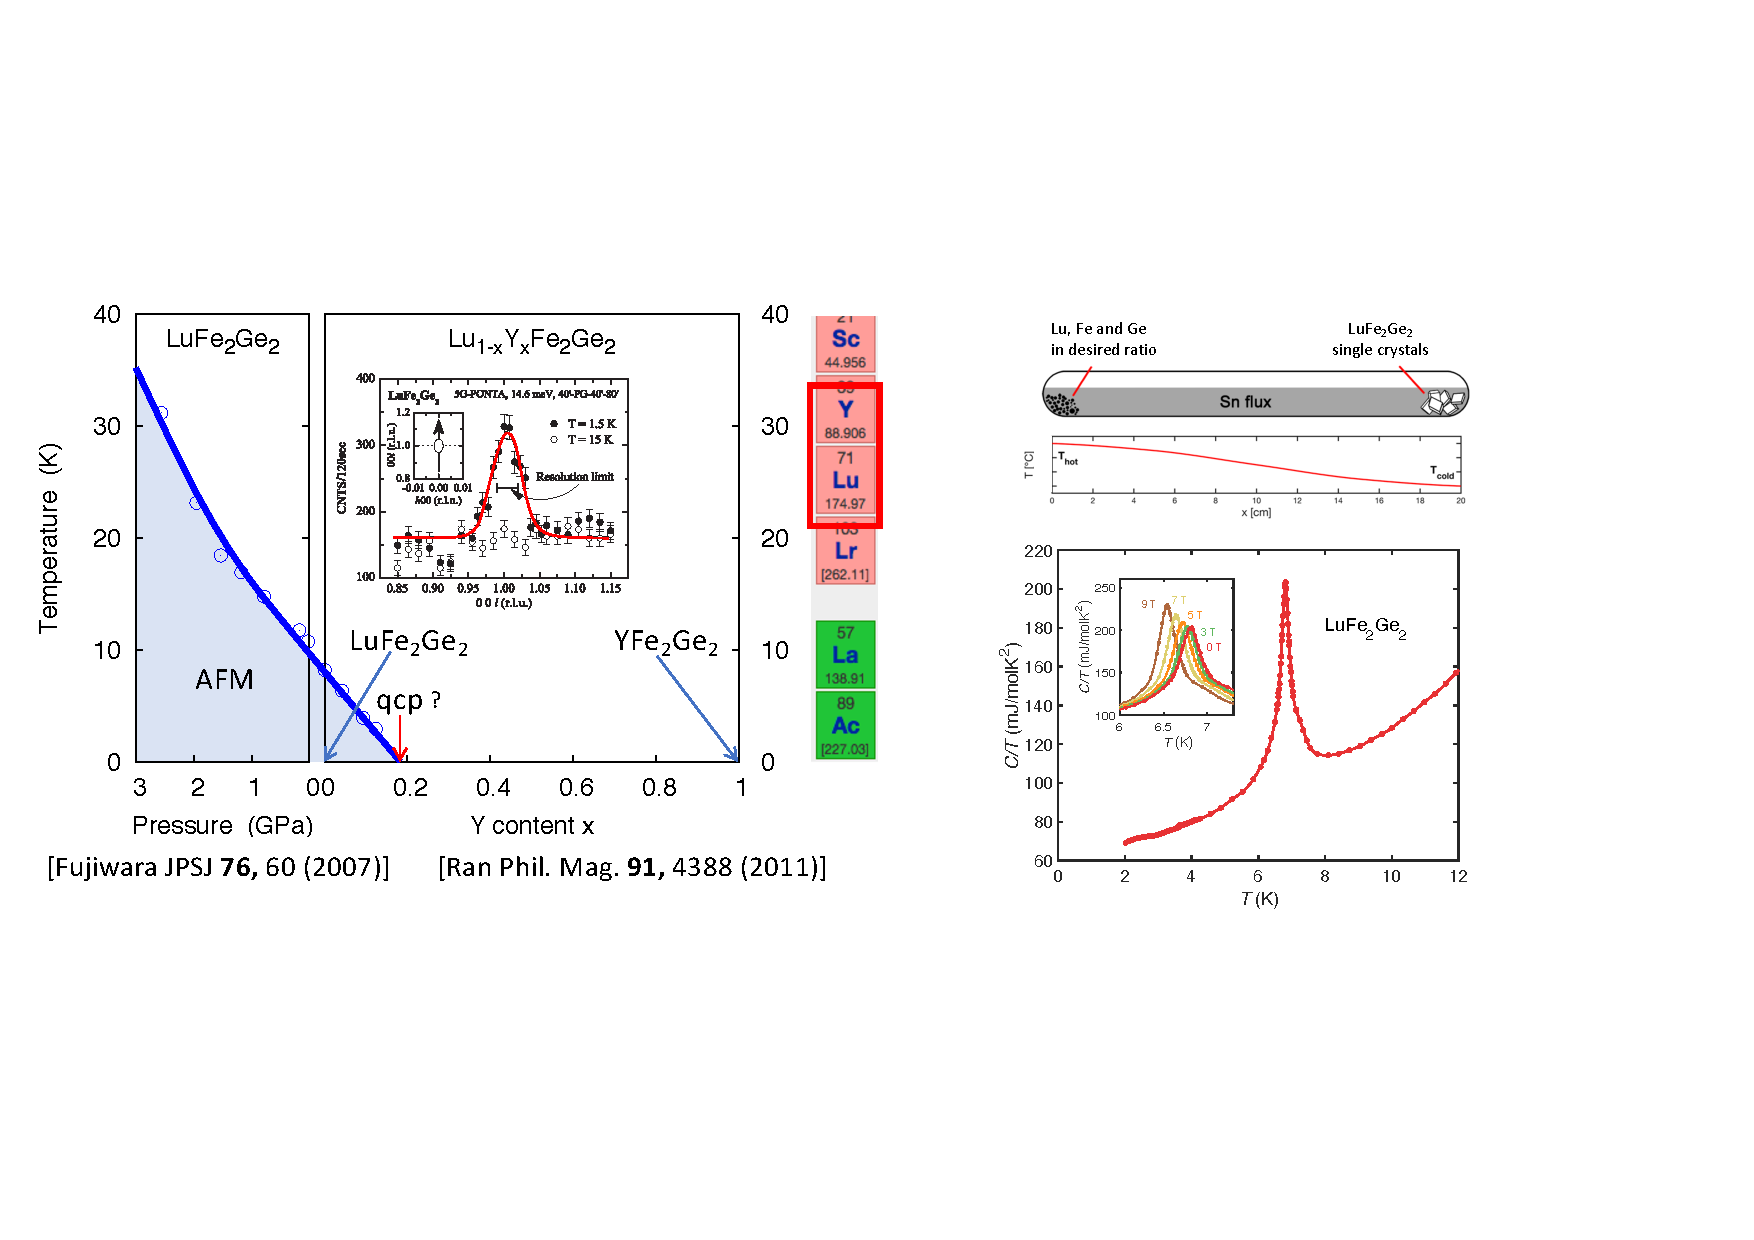
\includegraphics[width=0.9\columnwidth]{IntroPicture}}

\begin{itemize}
\item
Iron germanide superconductor YFe$_2$Ge$_2$ and substitution series with  Lu.
\item
SDW order in LuFe$_2$Ge$_2$.
\item
Evidence for superconductivity in LuFe$_2$Ge$_2$.
\end{itemize}
%\begin{columns}[t]
%\column{0.5\textwidth}
%Narrow electronic bands
%\begin{enumerate}
%\item
%Mott transition in NiS$_2$ \\
%{\scriptsize %S. Friedemann {\it et al.} Sci. Rep. {\bf 6,}  416 (2016), \\ 
%Semeniuk  arXiv: 2202.04024 (2022)}
%
%\item
%Mass renormalisation in YFe$_2$Ge$_2$ \\
%{\scriptsize Baglo  Phys. Rev. Lett. {\bf 129,} 046402 (2022)}
%
%\end{enumerate}
%
%%\column{0.5 \textwidth}
%Dissipation
%\begin{enumerate}
%\setcounter{enumi}{2}
%\item
%Structural qcp \\
%{\scriptsize L. Klintberg Phys. Rev. Lett. {\bf 109,} 237008 (2012), \\ S. Goh Phys. Rev. Lett. {\bf 114,} 097002 (2015)}
%
%\item
%Quasiperiodic structures \\
%{\scriptsize P. Brown Sci. Adv. {\bf 4:}eaao4793 (2018)}
%\end{enumerate}
%
%%\end{columns}
%%
%%\begin{columns}[t]
%%\column{0.25\textwidth}
%%\centerline{~}
%%\column{0.5\textwidth}
%%\centerline{~}
%Some of both 
%\begin{enumerate}
%\setcounter{enumi}{4}
%\item The Kondo lattice system CeSb$_2$ \\
%{\scriptsize O. Squire arXiv:2211.00975 (2022)}
%\end{enumerate}

%\end{columns}
% \visible<4->{
% \centerline{Quantum degeneracy temperature for electrons in metals: }
% \[
% T_F \sim ~\frac{\text{(density)}^{2/3}}{\text{mass}} \simeq 10,000 ~\text{degrees}
% \]
% }
%\begin{itemize}
%\item
%Bi-III: incommensurate high pressure structure.
%
%% \item Sliding mode $\rightarrow$
%% strong-coupling superconductivity
%
%\item
%YFe$_2$Ge$_2$: Iron-based superconductor with high $C/T \simeq 100~\text{mJ/molK}^2$.
%
%% \item 
%% New generation of high quality crystals show strong similarity to KFe$_2$As$_2$
%
%\end{itemize}
%
%\vspace{-1 em}
%\centerline{\makebox[\linewidth]{\rule{0.85\textwidth}{0.4pt}}}
%%%\centerline{\scriptsize L. Klintberg Phys. Rev. Lett. {\bf 109,} 237008 (2012), S. Goh Phys. Rev. Lett. {\bf 114,} 097002 (2015)}
%% \centerline{\scriptsize P. Brown Sci. Adv. {\bf 4:}eaao4793 (2018), S. Chen J. Phys. Mater. {\bf 3,} 015007 (2020)}
%% \centerline{\scriptsize S. Friedemann {\it et al.} Sci. Rep. {\bf 6,}  416 (2016), Semeniuk {\it et al.} arXiv: 2202.04024 (2022)}
%\centerline{\scriptsize J. Chen PRL {\bf 116,} 127001 (2016), PRB {\bf 99,} 020501(R) (2019)}

\end{frame}
%%%%%%%%%%%%%%%%%%%%%%%%%%%%%%%%%%%%%%%%%%%%%%%%%%%%%%%%%%%%%%%%%%%%%
% \begin{frame}[plain,label=TitlePage]
% \frametitle{Quantum Matter group}
% \hspace{5em}\includegraphics[width=1.2\columnwidth]{\Figures/GroupAdvertising/GruppenBilder2018}

% \end{frame}







%%% Local Variables: 
%%% mode: latex
%%% TeX-master: "GroTalk.ho"
%%% End: 
